\documentclass[12pt]{article}
\parskip=\bigskipamount
\parindent=0pt

\usepackage [autostyle, english = american]{csquotes}
\MakeOuterQuote{"}

\usepackage[utf8]{inputenc}
\usepackage{geometry}[margin=1in]
\usepackage{amsmath, amssymb}
\usepackage{tikz}
\usetikzlibrary{shapes, backgrounds}
  \usetikzlibrary{positioning}
  \usetikzlibrary{tikzmark}
  \usetikzlibrary{arrows}
  \usetikzlibrary{calc}
\usepackage{natbib}
\usepackage{listings}
\usepackage{minted}
\usepackage{changepage}
\usepackage{pgfplots}
\usepackage{caption}
\usepackage{subcaption}
\usepackage{float}
\usepackage{physics}

\newcommand{\R}{\mathbb{R}}

\title{\textbf{CLASSIFICATION METHODS FOR SUPPORT VECTOR MACHINES}}
\author{\textbf{JULIA ANDRONOWITZ} \\ B.S., Mathematics}
\date{May 2023}

\begin{document}

\maketitle
\thispagestyle{empty}

\begin{adjustwidth}{0.5in}{0.5in}
\begin{abstract}
    The purpose of this thesis is to give an introduction to the concept of Support Vector Machines in Machine Learning. We will first outline the idea of classification, including the maximal margin classifier and the support vector classifier. Examples of each will be given using programming languages such as R and Python. Then, we will move onto support vector machines and the use of kernels with example data. We will implement the techniques previously described in a real data set and finish by discussing applications of SVMs and examining the documentation of the support vector machine modules in R and Python.
\end{abstract}
\end{adjustwidth}

\vfill

\begin{center}
    University of Connecticut \\ Department of Mathematics \\ Advisor: Dr. Jeremy Teitelbaum
\end{center}

\newpage

\section*{INTRODUCTION}

The first discoveries regarding machine learning date back to the 1950s. Known as the "Turing Test", mathematician Alan Turing attempted to discern if a computer could fool a human into thinking it is also a human \cite{mlhistory}. In the years to follow, computer codes turned into learning programs that evolved the more times the code was run. In 1957, the first neural network was created which simulated a human brain's thought process. Ten years later, a basic pattern recognition algorithm was created called the "nearest neighbor" algorithm. Come the 1990's, accessibility to computers and advances in computers has exponentially increased. Scientists begin using a data-driven approach as large amounts of data are available, which allows computer algorithms to analyze data and learn from their results. Fast forward a few decades and we now have deep learning, survival analysis, and unsupervised learning.

Machine learning algorithms fall into one of two categories: supervised or unsupervised learning. Essentially, unsupervised learning arises when each observation does not have an associated response. This allows the machine to find certain patterns among the data and draw conclusions. Types of unsupervised learning include clustering and association. Clustering problems involve grouping the data based on the features. It is unknown how many groups are present in the data set when we begin, and so we rely on the machine to distinguish between groups. For example, we may want to group different animals based on their hunting/gathering methods and what they consume. Perhaps some animals tend to graze, others tend to scavenge, and others hunt. The algorithm would try to split the data into these three groups. In contrast, association rule learning problems focus on generalized trends between the groups. These types of trends are widely applicable to large portions of the data. For example, if one animal tends to graze on grass and other plants, the machine might suggest that another animal who grazes on grass will also eat other plants. Another common example is that people who buy one product are likely to buy another product \cite{supvunsup}.

\begin{figure}[h]
    \centering
    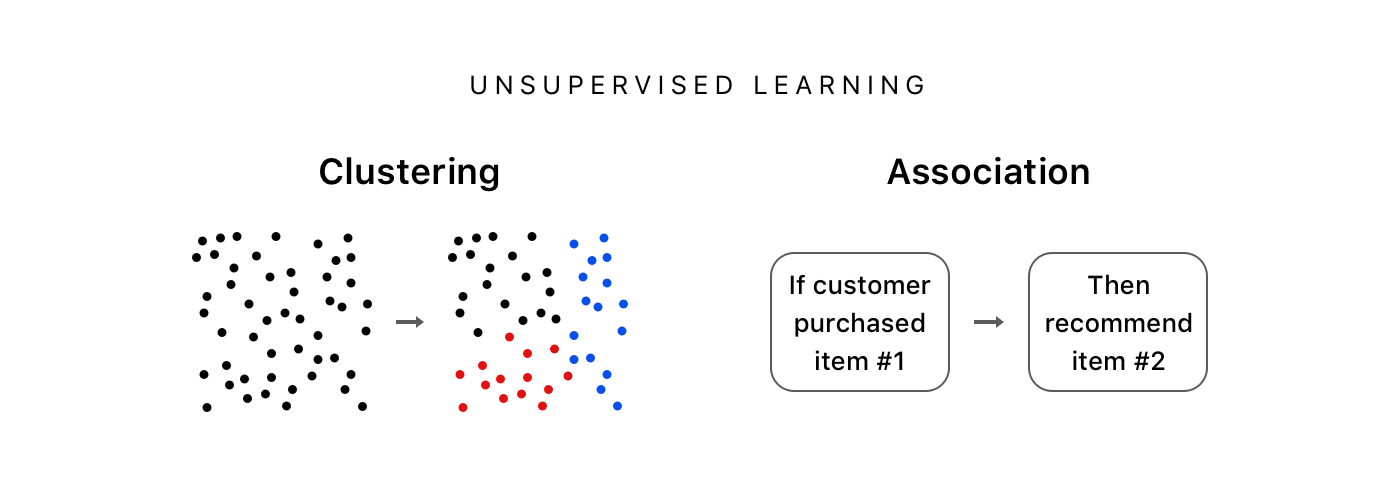
\includegraphics[height=2in]{clustering_v_association.png}
    \captionsetup[subfigure]{labelformat=empty}
    \begin{subfigure}[]{0.5\textwidth}
         \centering
         \caption{Source: Data Driven Investor}
     \end{subfigure}
    \label{fig1}
\end{figure}

In contrast, supervised learning uses data that is well-labeled to teach our model and either infer or predict. Inference problems aim for a better understanding of the relationship between the response variable and the features. On the other hand, prediction problems relate to developing a model that accurately fits the response variable to the predictors. Each observation in a data set has associated predictors and a response variable. Predictors are the input variables and can go by a variety of names such as variables, independent variables or features \cite{introstatlearning}. Predictors usually correspond to the variables $x_1,x_2,...,x_n$ where each $x_n$ is an input variable. The response variable is the dependent variable or what we are trying to measure, usually denoted as $y$. Let's take a look at some penguin data, shown in Table ~\ref{tab1}.

\begin{table}[h]
    \centering
    \begin{tabular}{p{1.8cm}p{1.8cm}p{1.8cm}p{1.8cm}p{1.8cm}p{1.8cm}p{1.8cm}}
         Culmen Length & Culmen Depth & Flipper Length & Body Mass & Delta 15 N & Delta 13 C & Species \\
         (mm) & (mm) & (mm) & (g) & (o/oo) & (o/oo) \\
         \hline
         50.2 & 18.7 & 198 & 3775 & 9.39305 & -24.25255 & Gentoo \\
         39.5 & 17.4 & 186 & 3800 & 8.94956 & -24.69454 & Adelie \\
         44.9 & 13.8 & 212 & 4750 & 8.11238 & -26.20372 & Chinstrap \\
         52.2 & 17.1 & 228 & 5400 & 8.36701 & -25.89834 & Chinstrap \\
         50.8 & 19 & 210 & 4100 & 9.98044 & -24.68741 & Gentoo \\
         42.5 & 20.7 & 197 & 4500 & 8.67538 & -25.13993 & Adelie
    \end{tabular}
    \caption{Penguin Data}
    \label{tab1}
\end{table}

In this example, the culmen length, culmen depth, flipper length, body mass, Delta 15 N and Delta 13 C are the predictors. Based on these variables, we want the model to predict which species the penguin is. So, each body measurement is a predictor and the species is the response variable. In supervised learning, we often have training and testing groups for our data. Training and test groups are a common practice in machine learning to both classify existing data points and assess the underlying accuracy of the model on known data. Training data is data used to teach our model how to estimate the response variable. Once the model is trained, we can apply the algorithm to the testing data which the model has not previously seen. Since we already have the response variable for this set in the original data, we can compare the model's predicted $y$-values, denoted $\hat y$, with the actual $y$-values. In machine learning, it is common to see the data split into about 80\% training and 20\% testing data, but these values can be manually specified in the code \cite{trainingvtest}. Suppose we collect the data for the ten students at the end of the year. Then, we have all their test scores for the year. We take 8 students and train the model based on these observations. Then, we use the remaining two students as the test set. 

Supervised learning can be categorized into either regression or classification problems. Generally, this has to do with the fact that data is either qualitative (categorical) or quantitative (numerical). Regression typically uses a quantitative response variable. In regression, we aim to create a model that uses features to accurately predict the response variable. We may want to see how a population's access to clean drinking water impacts their average life expectancy. Linear regression can be used in this case to see whether a correlation between the two variables exist and how strong that correlation is. We can also look at how accurate the model is at predicting the response variable as well as investigate whether the relationship is linear or non-linear. On the other hand, classification is common with a quantitative response variable. In these types of problems, the data is grouped into specific categories based on the given features. The model then is able to predict the category of an unknown data point. Similarly, we can also use tools to predict the accuracy of the model and determine if the relationship is linear or non-linear.

Developed in the 1990s, support vector machines are an approach to classification problems now widely used among data scientists. In the following paper, we will discuss what a support vector machine is, how one can be implemented among a data set and practical applications of SVMs.

\section*{HYPERPLANES}

We first begin by defining a hyperplane. Specifically, a hyperplane is "a flat affine subspace of dimension $p-1$" in a $p$-dimensional space \cite{introstatlearning}. In the two-dimensional space, a hyperplane looks like a straight line bisecting the data points into two distinct groups. We call this data linearly separable, as the data can be separated into two distinct groups by the hyperplane. In three dimensions, we see the formation of a plane. In higher dimensions, it can be hard to visualize the hyperplane, but the concept still applies.

Mathematically, a hyperplane in $\R^2$ is the equation $0=\beta_0+\beta_1x_1+\beta_2x_2$. Note that this is the equation of a one-degree polynomial, or a straight line. In higher dimensional spaces, a hyperplane has the form $$0=\beta_0 + \beta_1 x_1 + \beta_2 x_2 + \cdot \cdot \cdot + \beta_p x_p$$ We can generalize the equation of a hyperplane to be $$f(x)=\beta_0 + \beta \cdot x$$ where $f(x)=0$ and $\beta$ is a non-zero vector $\beta=(\beta_1,\beta_2,...,\beta_p)$ in $\R^p$ in which the dot product of $\beta$ and $x$ is computed. For any $x=(x_1,x_2)^T$ where the equation holds, we say the point is on the hyperplane. However, points that do not lie on the hyperplane will have $$0 \ne \beta_0 + \beta \cdot x$$ Moreover, the points that have $0>\beta_0 + \beta \cdot x$ will lie on one side of the hyperplane while the points $0<\beta_0 + \beta \cdot x$ will lie on the other. In this, we can see the concept of linearly separability. In a data set that is linearly separable and each observation is in one of two distinct groups, the hyperplane will bisect the data points in such a way that every point in one group is greater than zero while every point in the alternate group is less than zero.

To examine a hyperplane in two dimensions, we generate two distinct groups of data using \textit{R}.

\begin{minted}{R}
    n <- 200
    x1 <- matrix(rnorm(n*2, 1,0.3), ncol=2)
    x2 <- matrix(rnorm(n*2,-1,0.3), ncol=2)
    x <- rbind(x1,x2)
\end{minted}

We first set $n=200$. This will be the length of our data set. Then, we use the function \textbf{rnorm} to generate a set of data points from the normal distribution with mean 1 and standard deviation 0.3. The matrix function transforms the 400 randomly generated points into a [200 x 2] matrix. The same is done for a second group, instead with mean $-1$ and standard deviation 0.3. The \textbf{rbind} function combines these two groups into one vector, namely $x$.

\begin{minted}{R}
    plot(x,xlab="",ylab="")
    abline(h=0,v=0,col="gray",lty="dotted")
    abline(a=0,b=-1,col="black",lty="dashed")
\end{minted}

Now, we plot the function. The \textbf{abline} functions add lines at $x=0$ and $y=0$ as well as add one such separating hyperplane. Figure ~\ref{fig01} shows the output.

\begin{figure}[H]
\begin{center}
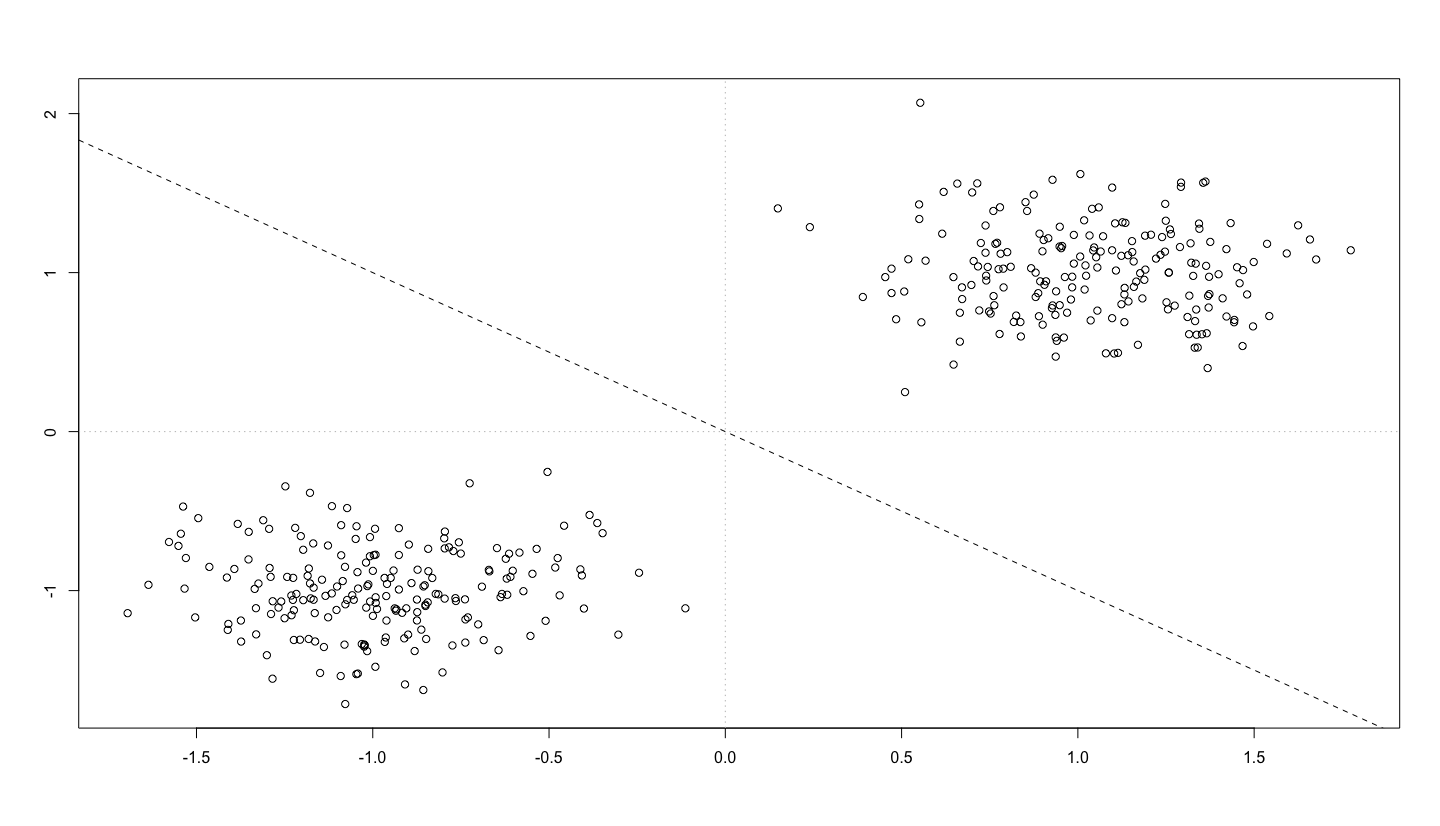
\includegraphics[width=5.5in]{fig02.png}
\caption{Randomly Generated Clustered Data \\ with Separating Hyperplane in $\R^2$}
\label{fig01}
\end{center}
\end{figure}


We see that there is a clear separation between the data points and a hyperplane that bisects the data. The equation of the hyperplane in this example is defined by $y=-x$. In the form $f(x)=\beta_0 + \beta \cdot x$, we have $f(x)=0$, $\beta_0=0$, and $\beta=(1,1)$ to give $0=0+x_1+x_2$ or $x_1=-x_2$.

Notice that we can rotate the line slightly in either direction and still have separating hyperplane. So long as the line does not pass through the points that the gray line intersects, there exist infinitely many such separating hyperplanes. An example is shown in red in Figure ~\ref{fig04}.

\begin{figure}[H]
\begin{center}
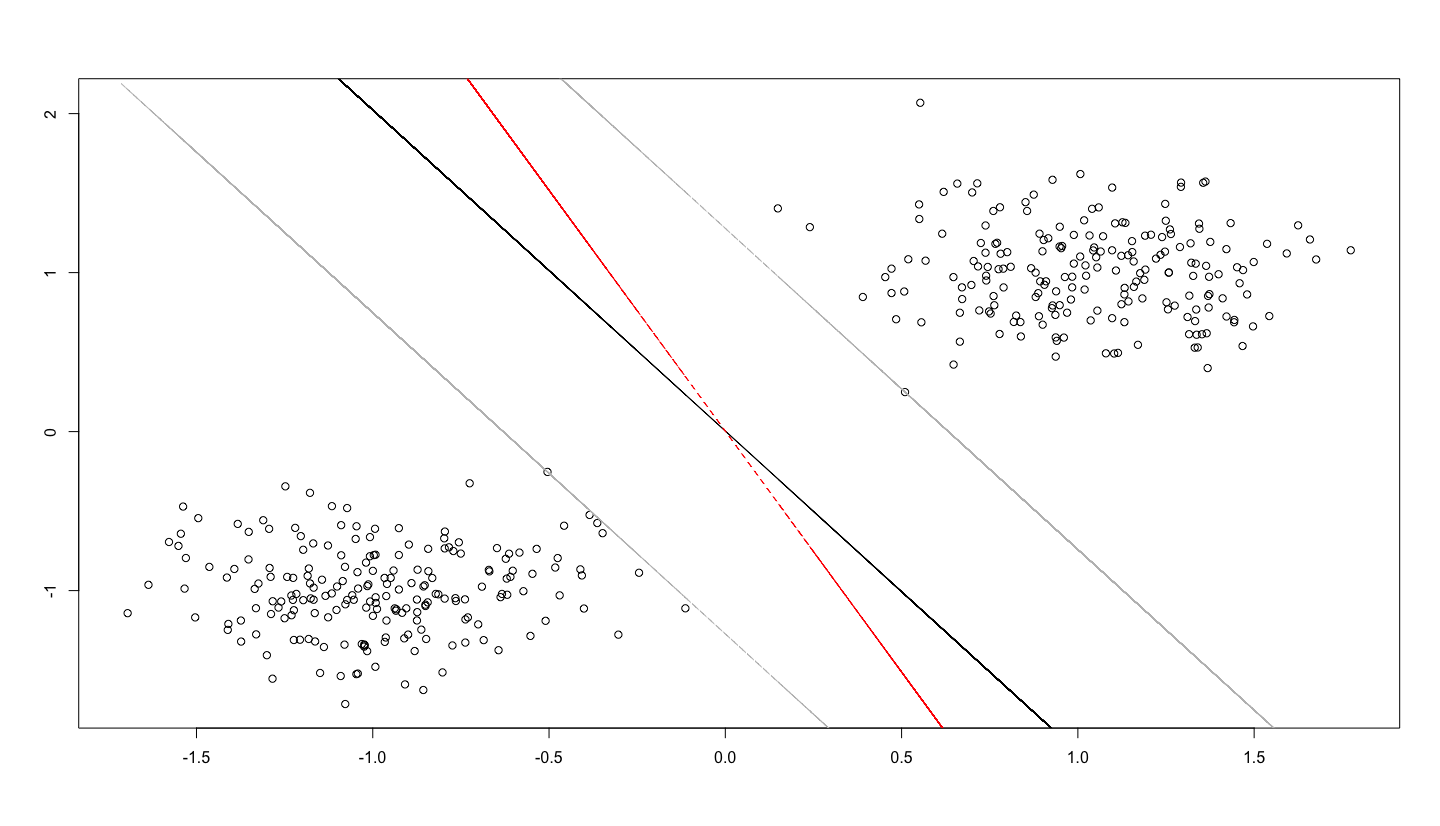
\includegraphics[width=5.5in]{fig03.png}
\caption{Randomly Generated Clustered Data with Multiple \\ Hyperplanes in $R^2$}
\label{fig04}
\end{center}
\end{figure}

Similarly, in a three-dimensional space the hyperplane partitions the data. A plane separates the set into two distinct groups. An example can be generated with Python. 

\begin{minted}{R}
    data1a = np.random.normal(-1,0.3,size=(10,1))
    data1b = np.random.normal(-0.5,0.3,size=(10,1))
    data1c = np.random.normal(0,0.1,size=(10,1))

    data2a = np.random.normal(1,0.3,size=(10,1))
    data2b = np.random.normal(0.5,0.3,size=(10,1))
    data2c = np.random.normal(0,0.1,size=(10,1))
\end{minted}

These functions set up our two data sets. The $a, b, c$ values correspond to the $x,y,z$ coordinates for each set. A randomly generated sample from the normal distribution is used. We then create the graph by setting up the axes and writing the equation for the hyperplane that will bisect the data before plotting the points.

\begin{minted}{python}
    x = np.linspace(-1, 1, 10)
    y = np.linspace(-1, 1, 10)

    x, y = np.meshgrid(x, y)
    eq = 1 * x + 0.15 * y

    fig = plt.figure()
    ax = fig.gca(projection='3d')
    ax.plot_surface(x, y, eq, color='green',alpha=0.3)

    ax.scatter(data1a,data1b,data1c, color='black')
    ax.scatter(data2a,data2b,data2c, color='black')

    plt.show()
\end{minted}

The output is shown in Figure ~\ref{fig02}.

\begin{figure}[H]
    \centering
    \includegraphics{fig04.png}
    \caption{Randomly Generated Clustered Data \\ with Separating Hyperplane in $\R^3$}
    \label{fig02}
\end{figure}

In this example, we see one set of points is to the left of the hyperplane while the other lies on the right. The equation of the hyperplane is $z = x + 0.15y$. In the form $f(x)=\beta_0 + \beta \cdot x$, we have $f(x)=0$, $\beta_0=0$, and $\beta=(1,0.15,-1)$ to give $0=0+x_1+0.15x_2-x_3$ or $x_3=x_1+0.15x_2$. Like in the two-dimensional case, there is an infinite number of separating hyperplanes in three dimensions. By slightly rotating the plane shown in Figure ~\ref{fig02} in either direction, we can visualize the concept of numerous other planes that would bisect the same data set.

\section*{MAXIMAL MARGIN CLASSIFIER}

The use of hyperplanes to distinguish between two classes is central to the maximal margin classifier. Also called the optimal margin classifier, this method aims to find the separating hyperplane that maximizes the distance between the two sets of points. That is, if the plane were to rotate slightly in either direction, it would be closer to the set of data points.

In the above example, we can classify each set of points to determine what side of the hyperplane they lie on. So, if $y_i=1$ then $0>\beta_0 + \beta \cdot x$ and if $y_i=-1$ then $0<\beta_0 + \beta \cdot x$. Each $y_i$ becomes the class label for that observation. Class labels are the identifiers for the data points and distinguish which class the observation belongs to. Introducing the following starred lines to our code produces colors in the graph according to the respective group:

\begin{minted}{R}
    n <- 200

    x1 <- matrix(rnorm(n*2, 1,0.3), ncol=2)
    x2 <- matrix(rnorm(n*2,-1,0.3), ncol=2)
    x<- rbind(x1,x2)

    y <- c(rep(1,n), rep(-1,n)) #**

    plot(x,xlab="",ylab="",col=(3-y)) #**
    abline(h=0,v=0,col="gray",lty="dotted")
    abline(a=0,b=-1,col="black",lty="dashed")
\end{minted}

The fifth line assigns a vector of 200 negative ones followed by 200 positive ones to the variable $y$. Combined with the adjusted plot function containing the color option $(3-y)$, the first 200 points are plotted blue and the last 200 points are plotted red. This gives out two groups shown in Figure ~\ref{fig05}.

\begin{figure}
    \centering
    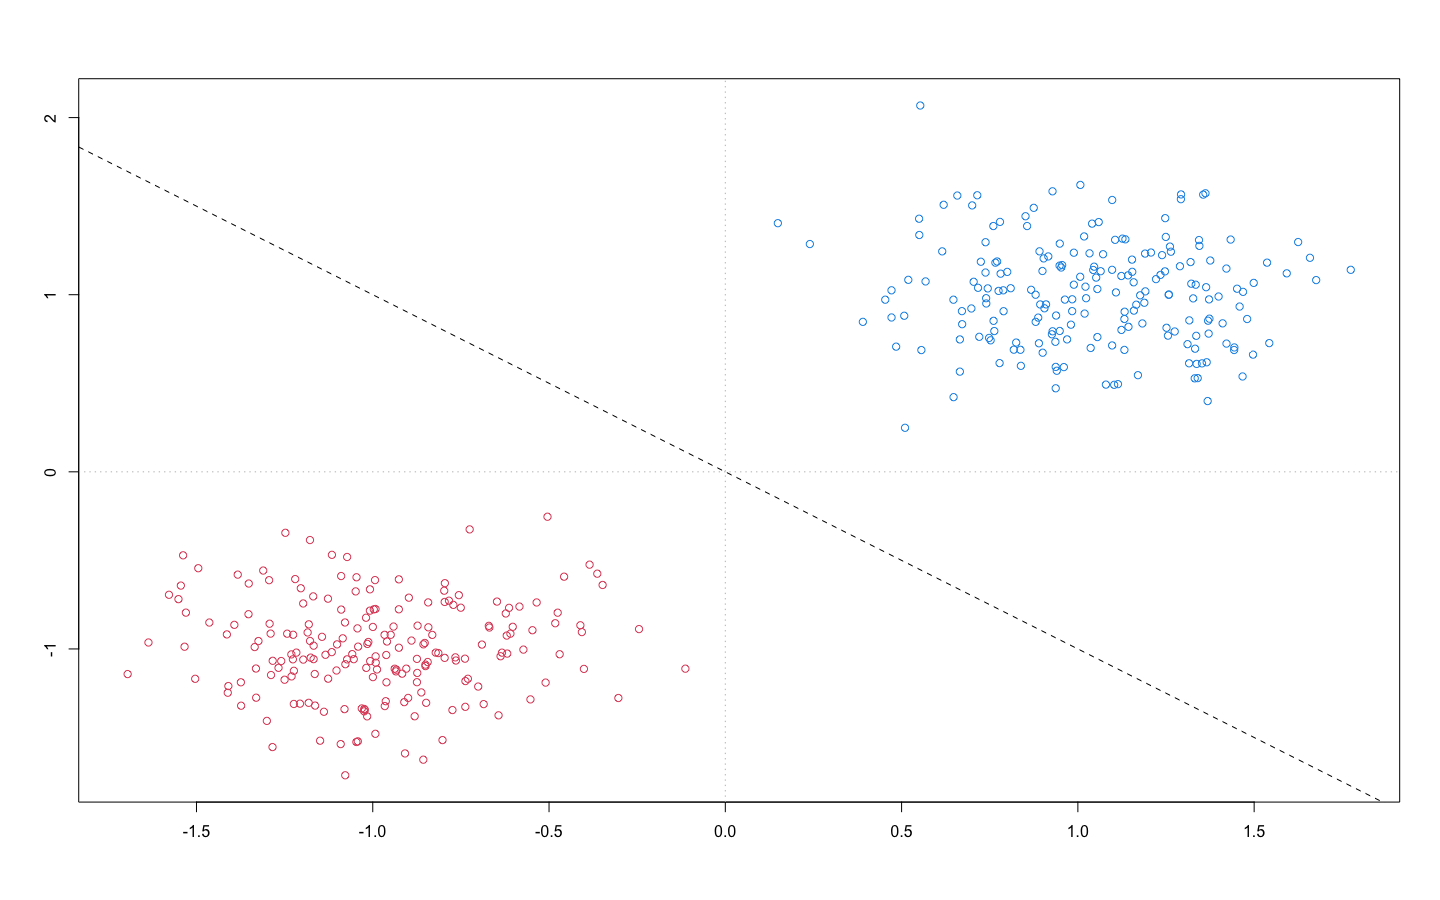
\includegraphics[width=5.5in]{fig05.png}
    \caption{Randomly Generated Data with Associated Class Label Coloring}
    \label{fig05}
\end{figure}

At this point, we know that points with $0>\beta_0 + \beta \cdot x$ will lie on one side of the hyperplane while the points $0<\beta_0 + \beta \cdot x$ lie on the other. Now that we have class labels, we see that points with $0<\beta_0 + \beta \cdot x$ have a class label $y_i$ of 1 while points with $0>\beta_0 + \beta \cdot x$ have a class label $y_i=-1$. Let those in the first class belong to the set $A^+$ and those in the second set belong to $A^-$, where $p \in A^+$ and $q \in A^-$. Combining these two constraints, we can produce one inequality such that

$$y_i(\beta_0+\beta_1x_{i1}+...+\beta_px_{ip})>0$$

The smallest such perpendicular distance from each observation to the hyperplane is known as the margin. Thus, we have the basic idea for the maximal margin classifier. We aim to maximize the margin $M$ to find the best separating hyperplane given by

$$y_i(\beta_0+\beta_1x_{i1}+...+\beta_px_{ip}) \ge M$$ 

We need to find the closest blue and red points such that shifting the hyperplane in any such way results in a smaller margin for either group. These points are known as the support vectors, as they are the only points that end up formulating the hyperplane. To do this, we must calculate the distance from the point to the plane. Suppose we look at a few points with a separating hyperplane of $0=\beta_0+\beta_1x_1+\beta_2x_2$.

\begin{figure}[h]
    \centering
    \label{supportvectors}
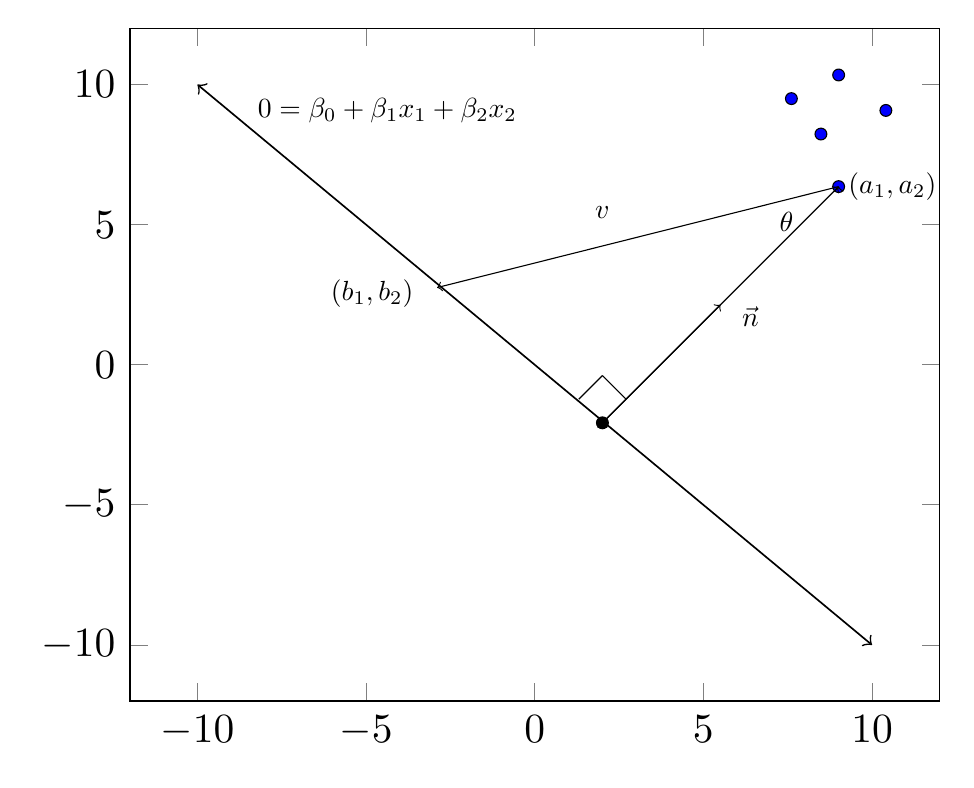
\begin{tikzpicture}[scale=1.5]
    \begin{axis}
            grid=both,
            axis equal,
            axis line style = [<->]
        ]
        \addplot[<->,domain=-10:10,samples=100]({x},{-x});
    \end{axis}
    \draw (1,5) node[right] {$0=\beta_0+\beta_1x_1+\beta_2x_2$};
    \draw (5.7, 4.055) node[left] {$\theta$};
    \draw (5.1,3.255) node[right] {$\vec{n}$};
    \draw (4,4) node[above] {$v$};
    \draw (2.05,3.25) node[above] {($b_1,b_2$)};

    \draw[fill] (4, 2.355) circle [radius = .05 cm];
    \draw[fill=blue] (6,4.355) circle [radius = .05 cm] node[right] {($a_1,a_2$)};
    \draw[fill=blue] (6.4, 5) circle [radius = .05 cm];
    \draw[fill=blue] (6, 5.3) circle [radius = .05 cm];
    \draw[fill=blue] (5.6, 5.1) circle [radius = .05 cm];
    \draw[fill=blue] (5.85, 4.8) circle [radius = .05 cm];
    
    \draw[->] (4, 2.355) edge (6,4.355);
    \draw[->] (4, 2.355) edge (5,3.355);
    \draw[->] (6,4.355) edge (2.6,3.5);
    \draw (4.2, 2.555) edge (4, 2.755);
    \draw (4,2.755) edge (3.8,2.555);
\end{tikzpicture}
    \caption{Diagram of Hyperplane and Support Vector}
\end{figure}

The perpendicular distance $\vec{n}$ from the point $(a_1,a_2)$ to the line can be written as $v\cos{\theta}$. This is equivalent to the dot product of $v$ and $\vec{n}$. We can find $\vec{n}$ by computing the normal vector to the line. 

$\expval{\beta_1, \beta_2}$, . By restricting the normal vector to a unit vector, we can feasibly find the points with the greatest margin. The unit vector $\vec{u}$ is calculated by dividing the vector by the norm $\frac{n}{||n||}$. This is equivalent to $$\frac{n}{\sqrt{\beta_1^2+\beta_2^2}}$$ So, by ensuring $\beta_1^2+\beta_2^2=1$ we confine the perpendicular distance to a unit vector. We can see how this translates to the hyperplane by taking the dot product of a point and $\vec{n}$
\begin{align*}
    (a_1-b_1,a_2-b_2) \cdot \expval{\beta_1,\beta_2} &= \beta_1a_1-\beta_1b_1+\beta_2a_2-\beta_2b_2 \\
    &= \beta_1a_1+\beta_2a_2-(\beta_1b_1+\beta_2b_2)
\end{align*}
Since $(b_1,b_2)$ lies on the hyperplane, $\beta_1b_1+\beta_2b_2=0$ and we are left with
\begin{align*}
    &=\beta_1a_1+\beta_2a_2 + \beta_0
\end{align*}
Thus, the hyperplane of the maximal margin classifier is given by

$$y_i(\beta_0+\beta_1x_{i1}+...+\beta_px_{ip}) \ge M$$ 

provided that

\begin{equation}\label{sumofsquares}
\sum_{j=1}^{p} \beta^2_j=1
\end{equation}

Though the maximal margin classifier is not a support vector machine quite yet, we may use the SVM module in the "e1071" library in $R$ to determine the equation of the line.

\begin{minted}{R}
    library(e1071)
    dat <- data.frame (x = x, y = as.factor (y))
    svmfit <- svm ( y~., data = dat , kernel="linear", cost = 1000, 
                scale = FALSE)
    plot(svmfit,dat)
\end{minted}

Once downloading the package, we assign the $x$ and $y$ variables to one dataframe. We convert the $y$ variable into a factor since class label is a binary value. In the \textbf{svm} function, the dataframe we just defined is the basis of the calculations. We assign the kernel as linear with a cost of 1000, though other options exist for non-separable data and non-linear decision boundaries which we will get to in later pages. We plot the function and see the output in Figure ~\ref{fig06}.

\begin{figure}
    \centering
    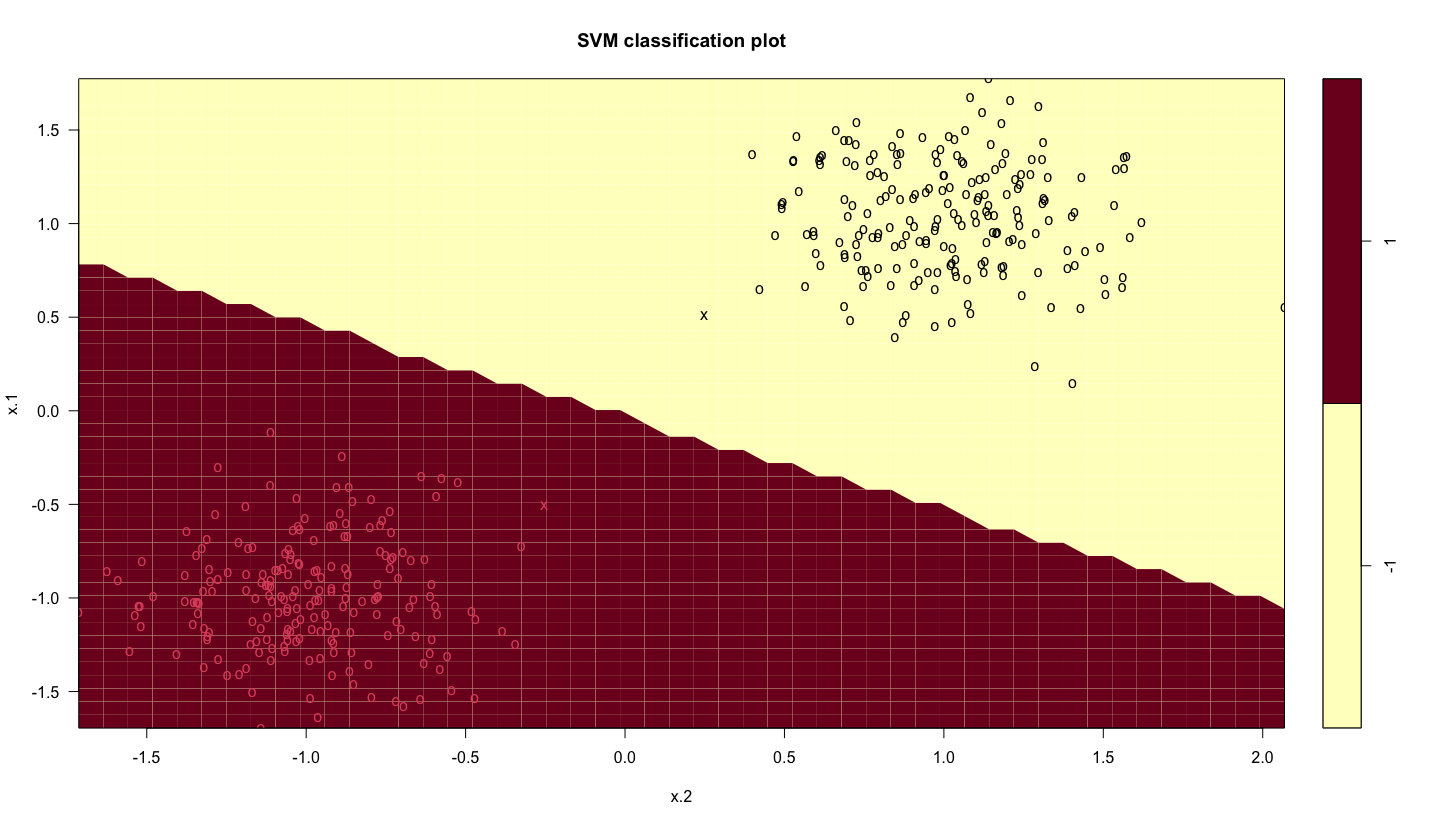
\includegraphics[width=5.5in]{fig06.png}
    \caption{Maximal Margin SVM Module Output in $R$}
    \label{fig06}
\end{figure}
As we see, the separating hyperplane is illustrated clearly albeit not pictured exactly linear. Details of the \textbf{svm} function can be found using the following:
\begin{minted}{R}
    summary(svmfit)
    svmfit$index
    svmfit$rho
    svmfit$coefs
\end{minted}

\begin{figure}[h]
    \centering
    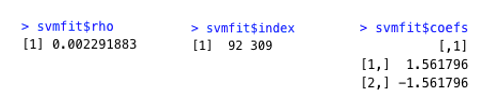
\includegraphics[width=5in]{svmfitoutput.png}
    \caption{Selected Output of SVM Function}
    \label{fig07}
\end{figure}

The \textbf{str} function tells us that \textbf{svmfit} is a list of 30 variables, some of which we defined in the function and others that were calculated. Particularly of interest are the \textbf{index}, \textbf{rho}, and \textbf{coefs} variables, which give the output in Figure ~\ref{fig07}. The \textbf{rho} variable is the intercept of the separating hyperplane, and the \textbf{coefs} variable is an array of the coefficients of the supporting vectors. The \textbf{index} variable tells us the indices of the observations that the classifier depends on, or the support vectors. In this case, it is data points 92 and 309. If we were to rotate the hyperplane in any direction, the margin from these two points to the black line would inevitably become smaller. Visually, we can see these two points as those that the supporting hyperplanes pass through in Figure ~\ref{fig08}.

\begin{figure}[h]
    \centering
    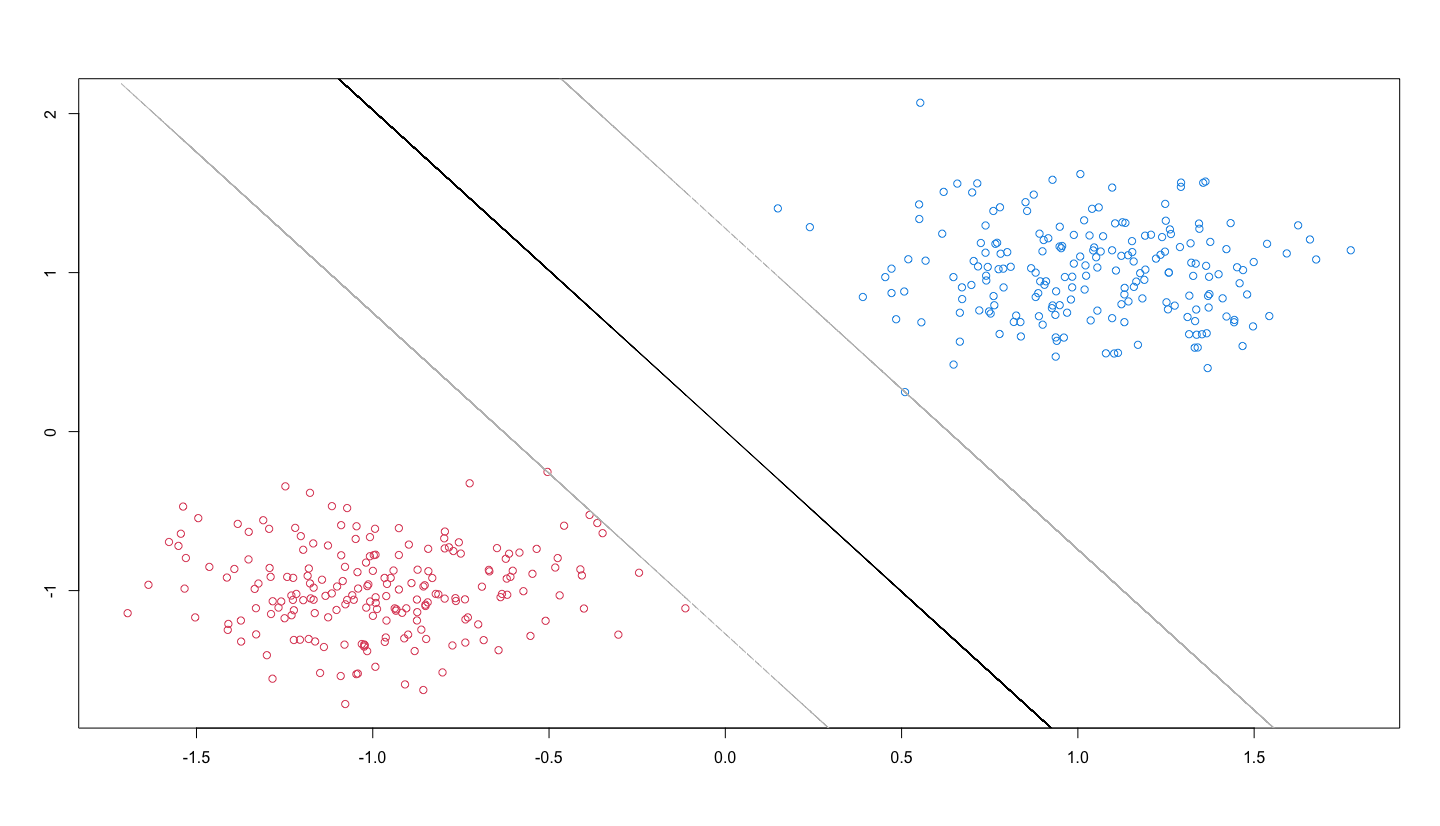
\includegraphics[width=5in]{fig08.png}
    \caption{Maximal Margin Classifier Output in $R$}
    \label{fig08}
\end{figure}

To find the equation of the line, we use the hyperplane function as outlined in \cite{teitelbaum2021svm}:
\begin{minted}{R}
    hyperplane <- function(P,data,x,z=0) {
      alphas <- -1*P$coefs
      svs <- data[P$index,]
      c <- P$rho - z
      a <- sum(t(alphas)*data[P$index,][1])
      b <- sum(t(alphas)*data[P$index,][2])
      (-c-a*x)/b
    }
\end{minted}
In this function, \textbf{P} is the \textbf{svm} function which we labeled \textit{svmfit}. The \textbf{data} is our dataframe containing the observations and class labels. \textbf{x} is the column vector of observations. We set \textbf{z}=0 for now, but this will later be shown to move the hyperplane vertically by a set constant. 

Inside the function, the \textbf{alphas} are assigned to the coefficients of the hyperplane and multiplied by negative one. The \textbf{svs} variable takes the index of the support vectors and finds the exact point values in the data. \textbf{c} refers to the intercept and can be adjusted by the variable \textbf{z}. The variables \textbf{a} and \textbf{b} take the $x$ and $y$ coordinates, respectively, of the support vectors and multiply by their corresponding coefficient, as calculated by taking the transpose of the \textbf{alphas} variable, then summed. In Python, the \textbf{hyperplane} function looks slightly different due to the differences in the corresponding module, but the concept remains the same.

\begin{minted}{Python}
    def hyperplane(P,x,z=0):
    """Given an SVC object P and an array of vectors x, computes the 
        hyperplane wx+b=z"""
    alphas = P.dual_coef_
    svs = P.support_vectors_
    c = P.intercept_[0]-z
    a = np.sum(alphas.T*svs,axis=0)[0]
    b = np.sum(alphas.T*svs,axis=0)[1]
    return (-c-a*x)/b
\end{minted}

The $R$ code for the plot referenced in Figure ~\ref{fig08} is below and pulls information from the \textbf{hyperplane} function.

\begin{minted}{R}
    plt0 <- hyperplane(svmfit,dat,x,0)
    plt1 <- hyperplane(svmfit,dat,x,1)
    plt2 <- hyperplane(svmfit,dat,x,-1)
    
    plot(x,xlab='',ylab='')
    lines(x,plt0,col='black')
    lines(x,plt1,col='gray',lty='dashed')
    lines(x,plt2,col='gray',lty='dashed')
\end{minted}

\section*{SUPPORT VECTOR CLASSIFIER}
\begin{itemize}
    \item soft margin classifier
    \item introduction of costs/penalties
    \item non-linearly separable example
    \item svm module code
\end{itemize}

figure of non-linearly separable data

figure of data with soft margin

\section*{SUPPORT VECTOR MACHINES}
\begin{itemize}
    \item non-linear decision boundaries
    \item use of kernels
    \item multi-class data
\end{itemize}

\section*{EXAMPLE}
\begin{itemize}
    \item penguin/iris dataset: well-known example
    \item possible example with real implications
\end{itemize}

\section*{APPLICATIONS}

One such example, as presented in \textit{Intro to Statistical Learning with Applications in R} \citep{introstatlearning} is the use of support vector machines in genetic expression data. The \textit{Khan} dataset in the $ISLR2$ package of $R$ contains expression measurements for 2,308 genes from tissue samples of patients with one of four types of small round blue cell tumors. The data is then split up into training and test groups. There are 63 observations in the training set and 20 observations in the test set. It is not feasible to visually plot the data on a graph, as there is a very large number of features relative to the number of observations. However, due to the large number of features, it is easy to find a linearly separating hyperplane that predicts the type of cell tumor. As such, the SVM approach outlined in the textbook yields no data points that are misclassified in the training set and two test set errors. In this case, a support vector machine was used to classify and predict cancer types based on gene expression data.

In fact, SVMs are a popular choice in machine learning approaches to detecting cancer. Several studies have shown SVMs perform with great accuracy. Among those include the prediction of breast cancer using SVM and an extremely randomized trees classifier \cite{breastcancer}

Support vector machines have also been used in multi-class lung cancer classification \cite{lungcancer}.

\section*{ANALYSIS OF R AND PYTHON SVM MODULES AND DOCUMENTATION}

\begin{itemize}
    \item supporting documentation for each
    \item ease of use
    \item notes on function parameters
\end{itemize}

\newpage
\thispagestyle{empty}

\bibliography{references}
\bibliographystyle{plain}

\end{document}